\chapter{Query Optimization}

The optimizer is a key component of the Query Manager. Its role is to select the optimal physical plan to execute queries using the operators and data structures provided by the Storage Engine. This chapter will show how functional dependencies are used for not only relational schema design, but also for optimization.

\section{Query Processing and Execution}

In general, there are many strategies to execute a query, in particular when it is complex. The problem of optimizing a query is influenced by the fact that a query can be written in several equivalent ways, and relational algebra operators can be implemented using different physical operators.

Query processing is divided into four stages:
\begin{itemize}
    \item \textbf{Query analysis}, in which the correctness of the SQL query is checked, and the query is translated into its internal form, typically based on relational algebra;

    \item \textbf{Query transformation}, in which the logical plan is transformed into an equivalent one that provides a better query performance;

    \item \textbf{Physical plan generation}, in which alternative physical plans are generated and evaluated, of which the one with the lowest cost is chosen;

    \item \textbf{Query evaluation}, in which the chosen physical plan is executed.
\end{itemize}
Query transformation and Physical plan generation are often considered part of the same phase, and are called Query optimizer.

The most interesting transformations regard Distinct elimination, GroupBy elimination, Where-subquery elimination, and View elimination.

\section{Functional Dependencies}

\BoxDef{Functional Dependency}{
Given a relation schema $R$ and $X,Y$ subsets of attributes of $R$, a functional dependency $X \rightarrow Y$ (read as ``$X$ determines $Y$'') is a constraint such that, for every possible instance $r$ of $R$ and for any two tuples $t_1, t_2 \in r$:
\begin{equation*}
    t_1[X] = t_2[X] \implies t_1[Y] = t_2[Y] 
\end{equation*}
}
A functional dependency is \textbf{trivial} if the consequent contains attributes also found in the antecedent:
\begin{equation*}
    XY \rightarrow X
\end{equation*}
A functional dependency is \textbf{atomic} if the consequent is composed of only one attribute:
\begin{equation*}
    X \rightarrow A
\end{equation*}
A functional dependency $X \rightarrow A$ is \textbf{canonical} if:
\begin{equation*}
    X \rightarrow A
\end{equation*}
holds true, but
\begin{equation*}
    X' \rightarrow A, \ \forall X' \subset X
\end{equation*}
does not. Every non-trivial dependency also contains one or more canonical dependencies, obtained by removing extraneous attributes. \\
A \textbf{key} is a set of attributes $K$ such that:
\begin{equation*}
    K \rightarrow T
\end{equation*}
holds and is canonical. \\
The \textbf{union rule} states that:
\begin{equation*}
    X \rightarrow A_1 \dots A_n \iff X \rightarrow A_1, \dots, X \rightarrow A_n
\end{equation*}
To specify that an attribute has a constant value for all tuples, the rule used is:
\begin{equation*}
    \emptyset \rightarrow Y
\end{equation*}

\BoxDef{Logical Implication}{
Given a set of functional dependencies $F$ on a relation schema $R$, a functional dependency $X \rightarrow Y$ is derived (implied) from $F$ if every instance of $R$ that satisfies $F$ also satisfies $X \rightarrow Y$:
\begin{equation*}
    F  \vdash X \rightarrow Y
\end{equation*}
This property holds if $X \rightarrow Y$ can be derived from $F$ using any of \textbf{Armstrong's axioms}:
\begin{itemize}
    \item $Y \subseteq X \implies X \rightarrow Y$ (Reflexivity)
    \item $X \rightarrow Y, Z \subseteq T \implies XZ \rightarrow YZ$ (Augmentation)
    \item $X \rightarrow Y, Y \rightarrow Z \implies X \rightarrow Z$ (Transitivity)
\end{itemize}
}
To test whether a functional dependency is implied by a set of functional dependencies, the \textbf{closure} of the antecedent can be calculated.
\BoxDef{Closure of Attribute Set}{
Given a schema $R <T,F>$, and $X \subseteq T$, the closure of $X$ is:
\begin{equation*}
    X^+ = \{A_i \in T | F \vdash X \rightarrow A_i\}
\end{equation*}
}
The following theorem holds true.
\BoxDef{Theorem}{
\begin{equation*}
    F \vdash X \rightarrow Y \iff Y \subseteq X^+
\end{equation*}
}

Consider a query on a set of tables $R_1(T_1), \dots, R_n(T_n)$, such that no attribute name appears in two tables. After joining the tables and performing a Select, assuming the Where condition $C$ is in CNF, these dependencies hold on the final result:
\begin{itemize}
    \item $K_{ij} \rightarrow T_i \ \forall K_{ij}$ key of $T_i$;
    \item $\emptyset \rightarrow A \ \forall A=c$ in $C$;
    \item $A_i \rightarrow A_j$ and $A_j \rightarrow A_i$ $\forall A_i = A_j$.
\end{itemize}

\section{Eliminations}

\subsection{Distinct Elimination}

Distinct normally requires a physical plan with duplicate elimination, and data must be grouped, usually via a sort operation (which is expensive). A query with a Distinct clause is translated into a relational algebra expression with the projection and duplicate elimination operators. To decide whether this duplicate elimination operator is unnecessary, a functional dependency theory algorithm is used. Specifically, the following theorem is used:
\BoxDef{Theorem}{
Let $A$ be the set of attributes of the result and $K$ the union of the attributes of the key for every table used in the query. If $A \rightarrow K$, then the duplicate elimination is unnecessary.
}
To find out whether $A \rightarrow K$, the closure of $A$ is computed.

If the query contains a GroupBy clause, then the theorem holds for $G$ (the grouping attributes) instead of $K$.

\subsection{GroupBy Elimination}

GroupBy also usually requires a sort operation. A GroupBy can be eliminated if either each group only has one record, or if there is only one group. The first case can be tested for as seen for Distinct, since it's equivalent to checking if the result contains duplicates. For the second case, we must check that the value of the grouping attributes is the same for each tuple; this is done by verifying that the closure of the empty set ($\{\}^+$) contains all the grouping attributes. 

If aggregation functions are used, Count will be replaced by 1, and Min($A$), Max($A$), Sum($A$), and Avg($A$) will be replaced by $A$.

\subsection{Where-subquery Elimination}

This is one of the most common and important transformations. In general, to execute these queries, the optimizer will generate a physical plan for the subquery, which will be executed for each record processed by the outer query. We will assume all subqueries  have been converted to an equivalent form using Exists, and that no GroupBy appears in the subquery. Given a query in the form
\begin{figure}[H]
    \centering
    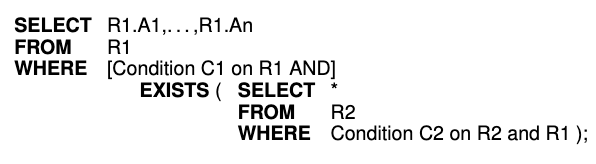
\includegraphics[width=0.75\linewidth]{img/opt_query1.png}   
\end{figure}
\noindent it is equivalent to
\begin{figure}[H]
    \centering
    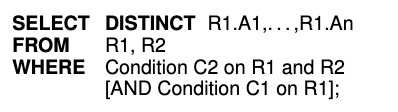
\includegraphics[width=0.5\linewidth]{img/opt_query2.png}
\end{figure}
The Distinct is necessary in the join form when a (1:N) relationship exists between R1 and R2. Note that if only a subset of R1's attributes appears in the Select clause, this transformation will not be correct unless the original query has a Distinct in the outer query.

If the subquery has an aggregation function, then the unnested equivalent requires a GroupBy clause on the projection attributes. A well-known problem is the \textbf{count bug problem}, which arises when the aggregation function is Count. In this case, the unnested query join must be replaced by an outer join.
An outer join is represented by a NATURAL RIGHT JOIN, NATURAL LEFT JOIN, or NATURAL FULL JOIN operator; the first one preserves all records from the left operand, the second one preserves all records from the right operand, and the third one preserves all records.

\begin{figure}[h]
\centering
    \begin{minipage}{0.49\textwidth}
    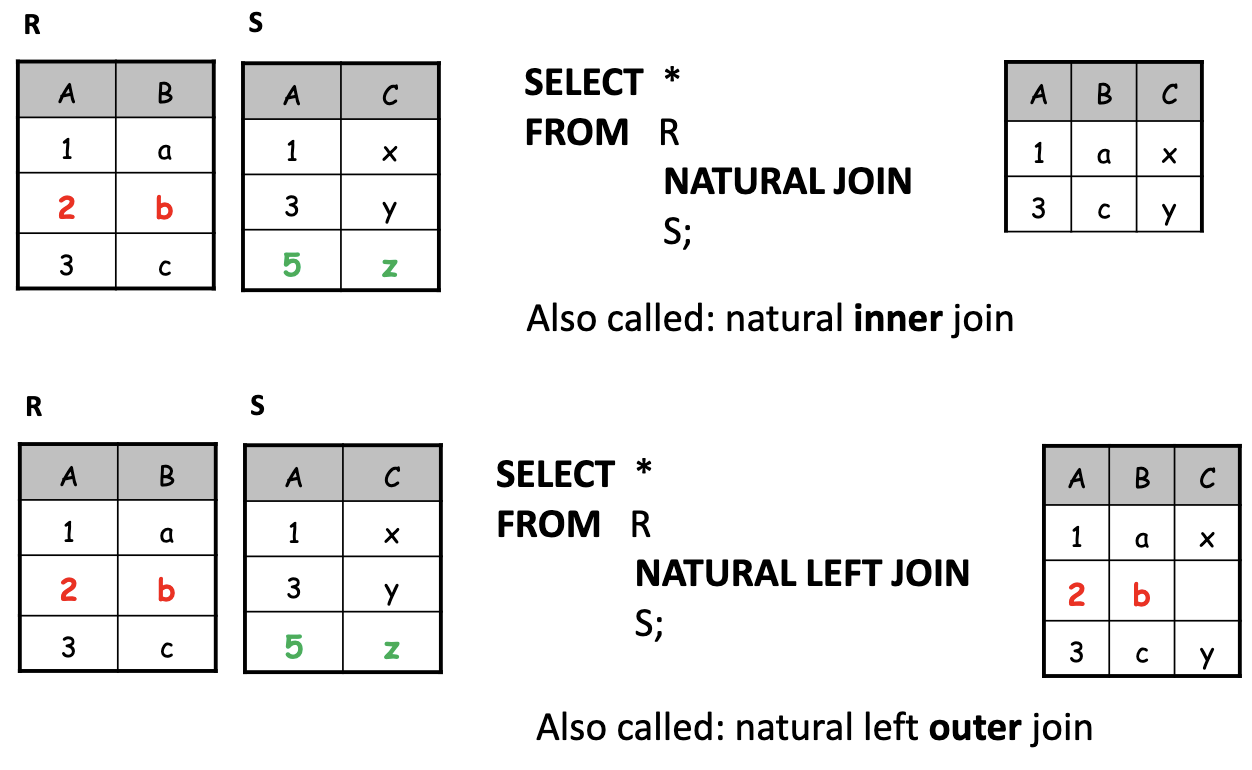
\includegraphics[width=\linewidth]{img/joins1.png}
    \end{minipage} 
    \hfill
    \begin{minipage}{0.49\textwidth}
    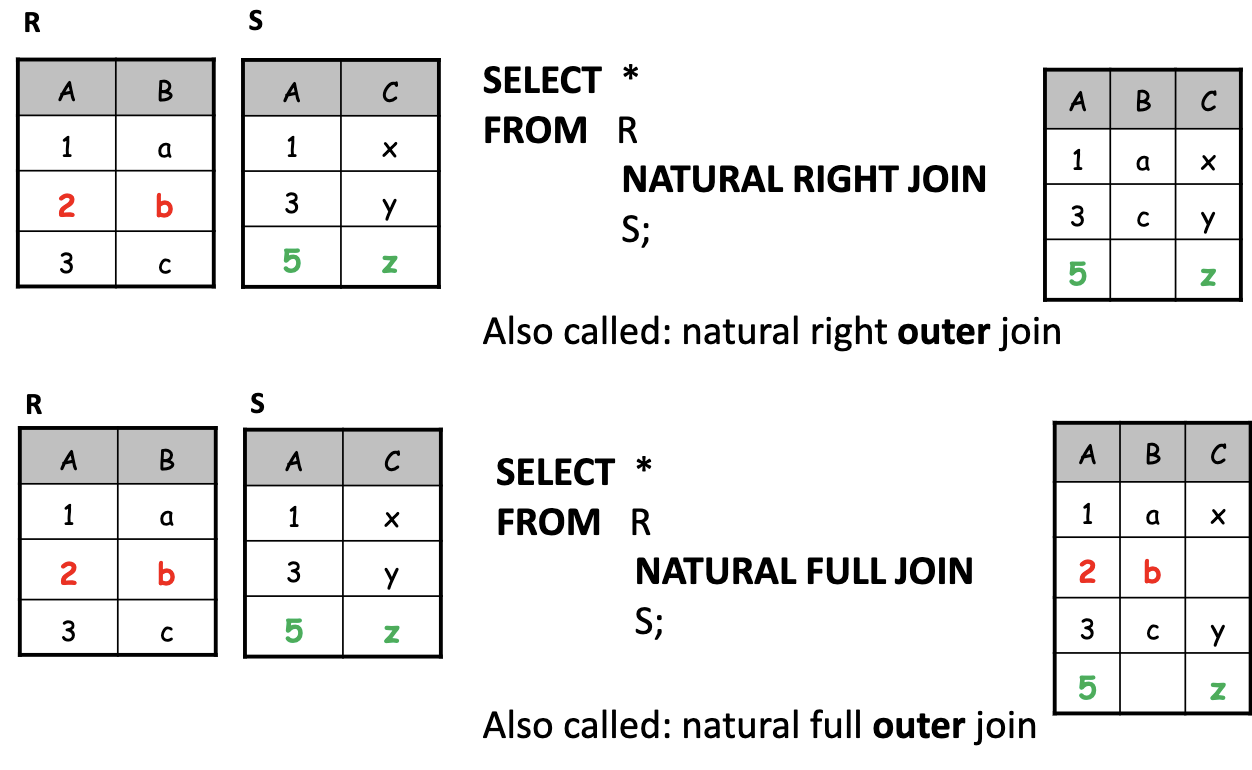
\includegraphics[width=\linewidth]{img/joins2.png}
    \end{minipage}
    \caption{Types of join.}
    \label{fig:joins_in_out}
\end{figure}

\subsection{View Merging}

Complex queries are easier to understand if views are used. The With clause defines temporary views available only to the query in which the clause occurs. When a query generates a view, the optimizer generates a physical sub-plan for the Select that defines the view, and optimizes the query considering the scan as the only operation available for the result of the view; with this technique, the view is optimized separately from the rest of the query.

In the logical plan, the transformation is made by replacing the reference to a view name with the corresponding logical plan. The new logical plan is then rewritten using equivalence rules of relational algebra to put it in the following canonical form:
\begin{equation*}
    \pi^b(\sigma(\gamma(\sigma(^{\bowtie}_J R_i))))
\end{equation*}
The transformation of a query to avoid the use of views defined with a GroupBy generally requires pulling the GroupBy above a join, using the following algebraic equivalence rule:
\begin{equation*}
    ({}_{X_R} \gamma_F(R)) \bowtie_{f_{k} = p_k} S \equiv {}_{X_R \cup A(S)} \gamma_F (R \bowtie_{f_{k} = p_k} S) \,,
\end{equation*}
where $X_R$ is a set of attributes of $R$, $f_k \in X_R$ the foreign key of $R$, and $p_k$ the primary key of $S$ of attributes $A(S)$.

\section{Physical Plan Generation}

With eliminations, a ``random'' physical plan is generated for the query, which is then optimized. Generation, on the other hand, directly finds the best possible physical plan, in two steps: generation of alternative physical query plans, and choice of physical query plan with the lowest estimated cost. To estimate the cost of the entire plan, it is necessary to estimate the cost of the physical operator and the size of the result of every node in the tree (in a bottom-up fashion). The following sections will show how to choose the physical query plan of minimum cost for different types of queries.

\subsection{Single-Relation Queries}

For these queries, the only question to solve is whether to use indexes when accessing the data instead of performing a simple TableScan. Some relations may have single or multiple indexes defined on one or more of their attributes; in that case, the cost of reading the entire table is compared against the cost of reading the index and retrieving the data using the RIDs contained in the index. Usually, using an index is better if the selectivity factor of the query is restrictive enough. A special case happens when the attributes appearing in the Select are included in the prefix of the key of an index of the relation; the query can be evaluated by only reading the index itself, which is much faster than reading the whole table. 

\subsection{Multiple-Relation Queries}

The most important issue in these queries is the order in which the relations are joined. Every permutation of relations yields the same result but corresponds to a different plan; given $n$ relations, there are $n!$ different permutations, each of which generates a huge number of candidates depending on the specific joins performed in the plan. Additionally, there are different choices for the specific physical operator used to implement the join, increasing the total number of possible plans.

The full search in the space of candidates starts by finding which relation is cheaper to access (representing the operator as a standalone plan). Then, the second cheapest plan is chosen among the ones not selected in the previous step and the ones that would be generated by a join of the previously chosen relation with a different one, and so on until the entire query is covered by the physical plan. At each step, the only plans evaluated are the ones behind a so-called ``frontier'', meaning all plans that are direct children of either the (empty) root of the entire search or a plan that has been selected as a minimum cost one.

This algorithm can be incredibly efficient for simpler queries and incredibly slow for complex ones. In the latter case, the algorithm will tend to backtrack to higher levels in the ``tree'' of physical plans explored. A simple pseudocode for this algorithm is presented below.

\begin{algorithm}
\caption{Full search pseudocode.}
\begin{algorithmic}[1]
    \State Initialize $Plans$ to the best plans to access each relation in the query.
    \Loop
        \State Extract the fastest plan $P$ from $Plans$.
        \If{$P$ is complete}
            \State \Return $P$
        \EndIf
        \For{$R$ not in $P$}
            \State Put the best plan between $P \bowtie R$ and $R \bowtie P$ in $Plans$.
        \EndFor
        \State Remove $P$.
    \EndLoop
\end{algorithmic}
\end{algorithm}

Several heuristics have been proposed that can help speed up the algorithm, meaning that the algorithm may not find the optimal physical plan but one that is good enough. The most commonly used heuristics are:
\begin{itemize}
    \item \textbf{Limitation in the number of successors}: each permutation is evaluated by associating the join operators only to the left, creating \textbf{left-deep} trees, where each node from the root up until the second-to-last level has a join as a left child and a relation as a right child (as opposed to \textbf{right-deep} and \textbf{bushy} trees). A left-deep tree has the advantage of allowing the use of an index nested loop join operator. 

    \begin{figure}[h]
        \centering
        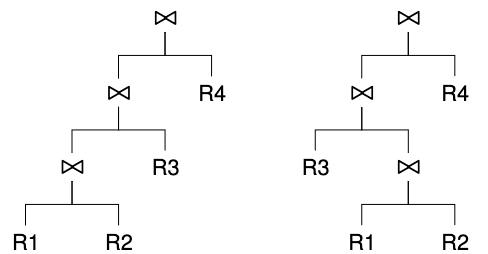
\includegraphics[width=0.5\linewidth]{img/leftdeep_vs_bushy.png}
        \caption{Left-deep tree on the left, bushy tree on the right.}
        \label{fig:ldeep-vs-bushy}
    \end{figure}

    \item \textbf{Greedy search}: once the logical node of minimum cost has been expanded, the other nodes are not considered anymore, avoiding any backtracking. In general, solutions found using a greedy search are suboptimal, but thanks to the fact that it is found in less time, this search is usually the default one used by DBMSs.

    \item \textbf{Iterative full search}: a possibility is to use a mixed approach. The full search is made up to a predetermined number of levels, then the best node to expand is chosen, and, as in the greedy search, the other nodes will not be considered any longer. The full search will continue for the predetermined number of levels, and so on.

    \item \textbf{Interesting orders}: when the merge-join operator is available, and the query result must be sorted because of the presence of an OrderBy or a GroupBy, it is useful to organize the search as follows: at each step, for each logical query subexpression, the preserved query plans will be the one with minimum cost as well as the best plans producing an interesting order of the records potentially useful for the final query plan. 
\end{itemize}

\subsection{Other Queries}

\subsubsection{Queries With GroupBy}

If the GroupBy is necessary, the optimizer produces a physical plan for the Select only, sorting the data on the grouping attributes; this plan is then extended with the physical operator for the GroupBy and the one for the Project over the Select attributes. If an Having clause was specified, the physical plan is also extended with a selection operator, and the GroupBy computes whatever aggregation function used in the Having and Select clauses.

\paragraph{Exchanging with a Join}
If the query requires a Join, it may be convenient to GroupBy before the Join (with the constraint that the GroupBy is done on the same attributes used in the Join); often, however, Joins are submultiplicative, so moving it above the GroupBy may make the plan more expensive. The equivalence rules for this transformation are done under these assumptions:
\begin{itemize}
    \item The tables do not have null values, and primary and foreign keys have only one attribute;

    \item The queries are a single Select with GroupBy and Having, but without any subselect, Distinct, or OrderBy clauses;

    \item The Select includes all grouping attributes.
\end{itemize}
Then, the pre-grouping problem is: when does this equivalence rule:
\begin{equation*}
    {}_X \gamma_F (R \bowtie_{f_k = p_k} S) \equiv (({}_{X'} \gamma_{F'}(R)) \bowtie_{f_k = p_k} S)
\end{equation*}
hold?

The fundamental condition is that the join is unary w.r.t. the attributes $X$, meaning that it produces exactly one record for each value of that attribute. This is true under the following conditions:
\begin{itemize}
    \item Let $C_j$ be the Join condition; then $C_j \vdash X \rightarrow A(S)$, producing one record from $S$ for every group;

    \item Each aggregate function only uses attributes from $R$.
\end{itemize}

\paragraph{Exchanging with a Filter}
For this transformation, we need to find if the following equivalence rule holds:
\begin{equation*}
    \sigma_{\phi}({}_X \gamma_F (E)) \equiv {}_X \gamma_F (\sigma_{\phi}(E))
\end{equation*}
This equivalence rule is typically used when the query contains an Having clause, or it uses a view that specifies a condition on its attributes. There's two possible cases; either the selection is done on the dimensions of a table, or it is done on the results of aggregate functions in the GroupBy. \\
The first case is simple:
\begin{equation*}
    \sigma_{\phi_X} ({}_X \gamma_F (E)) \equiv {}_X \gamma_F (\sigma_{\phi_X} (E))
\end{equation*}
If the restriction is done on the same attributes on which the GroupBy is performed, it can be moved below. However, this rule is rarely used, since these conditions are normally specified in the Where clause and not the Having clause, so they already appear below GroupBys. \\
The second case is more complicated:
\begin{equation*}
    \sigma_{\phi_F} ({}_X \gamma_{AGG(A_1) \ AS \ F_1, \dots, AGG(A_n) \ AS \ F_n} (E))
\end{equation*}
Equivalence rules can be built only in these two case
\begin{gather*}
    \sigma_{\phi_{Mb \geq v}} ({}_X \gamma_{MAX(b) \ AS \ Mb} (E)) \equiv {}_X \gamma_{MAX(b) \ AS \ Mb} (\sigma_{b} \geq v(E))\\
    \sigma_{\phi_{mb \leq v}} ({}_X \gamma_{MIN(b) \ AS \ mb} (E)) \equiv {}_X \gamma_{MIN(b) \ AS \ mb} (\sigma_{b} \leq v(E))
\end{gather*}